\solutionset

\begin{enumerate}

\item \textbf{Toomre Instability.}

\begin{enumerate}

\item Substituting in the perturbed terms for $\Sigma$, $\vecv$, and $\phi$, the linearized equation of mass conservation is
\begin{eqnarray*}
\frac{\partial}{\partial t}\left(\Sigma_0 + \epsilon \Sigma_1\right) + 
\nabla \cdot \left[\left(\Sigma_0 + \epsilon \Sigma_1\right) \left(\vecv_0 + \epsilon \vecv_1\right)\right] & = & 0 \\
\frac{\partial}{\partial t} \Sigma_1 + \Sigma_0 \nabla \cdot  \vecv_1 + \nabla \cdot \left(\Sigma_1 \vecv_0\right) & = & 0.
\end{eqnarray*}
In going from the first line to the second, we dropped terms of order $\epsilon^2$, we used the fact that $\Sigma_0$ is constant in time to drop the term $\partial\Sigma_0/\partial t$, and we used the fact that it is constant in space (since the unperturbed state is uniform) to take the $\Sigma_0$ factor out of the divergence. Note that $\vecv_0$ and $\Sigma_1$ are not constant in space, so they cannot be taken out of the divergence.

The linearized momentum equation is
\begin{eqnarray*}
\lefteqn{\frac{\partial}{\partial t}\left(\vecv_0 + \epsilon \vecv_1\right) + \left(\vecv_0 + \epsilon \vecv_1\right)\cdot \nabla\left(\vecv_0 + \epsilon \vecv_1\right)} \qquad \\
 & = & -\frac{\nabla (\Sigma_0+\epsilon \Sigma_1)}{\Sigma_0+\epsilon\Sigma_1} c_s^2 - \nabla (\phi_0 + \epsilon\phi_1)
\nonumber \\
& & {}
- 2\veco \times \left(\vecv_0 + \epsilon \vecv_1\right) + \Omega^2 (x \ehat_x + y \ehat_y). \\
\end{eqnarray*}
To simplify this, we recall that, since the equilibrium is an exact solution, it must be the case that
\begin{displaymath}
\frac{\partial}{\partial t} \vecv_0 + \vecv_0 \cdot \nabla \vecv_0 = -c_s^2 \frac{\nabla\Sigma_0}{\Sigma_0} - \nabla \phi_0 - 2\veco\times\vecv_0 + \Omega^2 (x \ehat_x + y \ehat_y),
\end{displaymath}
and we can therefore cancel these terms. Doing so, and dropping terms of order $\epsilon^2$, we are left with
\begin{displaymath}
\frac{\partial}{\partial t} \vecv_1 + \vecv_0 \cdot\nabla \vecv_1 + \vecv_1 \cdot \nabla \vecv_0
= - \frac{\nabla \Sigma_1}{\Sigma_0} c_s^2 - \nabla \phi_1- 2  \veco\times\vecv_1.
\end{displaymath}

Finally, the linearized Poisson equation is
\begin{eqnarray*}
\nabla^2 (\phi_0 + \epsilon \phi_1) & = & 4\pi G (\Sigma_0 + \epsilon \Sigma_1) \delta(z) \\
\nabla^2 \phi_1 & = & 4\pi G \Sigma_1 \delta(z).
\end{eqnarray*}
In deriving the second line we used the fact that the unperturbed state is an exact solution to cancel $\nabla^2 \phi_0$ with $4\pi G \Sigma_0\delta(z)$.

\item First, we plug the Fourier mode trial solutions into the Poisson equation:
\begin{displaymath}
 \phi_a \nabla^2 e^{i(kx-\omega t)-|kz|} = 4\pi G \Sigma_a e^{i(kx-\omega t)} \delta(z).
\end{displaymath}
To eliminate the $\delta(z)$, we now integrate both sides in $z$ over a range $[-\zeta,\zeta]$ and evaluate in the limit $\zeta \rightarrow 0$. This gives
\begin{eqnarray*}
\lefteqn{\phi_a \int_{-\zeta}^\zeta \left(\frac{\partial^2}{\partial x^2} + \frac{\partial^2}{\partial y^2} + \frac{\partial^2}{\partial z^2}\right) e^{i(kx-\omega t)-|kz|} \, dz} \qquad\qquad\qquad
\nonumber \\
& = &  4 \pi G \Sigma_a  e^{i(kx-\omega t)} \int_{-\zeta}^\zeta \delta(z) \, dz \\
& = & 4\pi G \Sigma_a e^{i(kx-\omega t)}.
\end{eqnarray*}
To evaluate the left-hand side, note that the $\partial^2/\partial y^2$ term vanishes because there is no $y$-dependence, and the $\partial^2/\partial x^2$ term will also vanish when we take the limit $\zeta\rightarrow 0$, because the integrand is finite. Only the $\partial^2/\partial z^2$ term will survive. Thus we have
\begin{eqnarray*}
4\pi G \Sigma_a & = & \phi_a \lim_{\zeta\rightarrow 0} \int_{-\zeta}^\zeta \frac{\partial^2}{\partial z^2} e^{-|kz|} \, dz \\
& = & \phi_a \lim_{\zeta\rightarrow 0} \left[\left(\frac{d}{dz} e^{-|kz|}\right)_{z=\zeta} - \left(\frac{d}{dz} e^{-|kz|}\right)_{z=-\zeta}\right] \\
& = & -2\phi_a |k|
\end{eqnarray*}
Thus we have
\begin{displaymath}
\phi_a = -\frac{2\pi G\Sigma_a}{|k|}.
\end{displaymath}

\item As a first step, let us rewrite the terms involving $\vecv_0$ in a more convenient form; this is the Taylor expansion part. Recall that we are in a frame that is co-rotating with the disk, and where $x$ is the distance from the center of our co-rotating reference frame in the radial direction. In the lab frame, the velocity is $\vecv_0' = v_R \ehat_\phi$, and the velocity of the co-rotating reference frame at a distance $r$ from the origin is $\vecv_{\rm rot} = \Omega_0 r \ehat_\phi$. The unperturbed velocity in the rotating frame is the difference between these two, i.e.,
\begin{eqnarray*}
\vecv_0 & = & \vecv_0' - \vecv_{\rm rot} \\
& = & \left(v_R - \Omega_0 r\right) \ehat_y \\
& = & \left[\Omega_0 R - \Omega_0 \left(R + x\right)\right] \ehat_y \\
& = & -\Omega_0 x \ehat_y,
\end{eqnarray*}
where we have used the fact that $\ehat_\phi$ in the lab frame is the same as $\ehat_y$ in our co-rotating frame.

With this result in hand, we can now begin to make substitutions into the perturbed equations. The perturbed equation of mass conservation becomes
\begin{displaymath}
-i\omega \Sigma_a + i k \Sigma_0 v_{ax} = 0.
\end{displaymath}
The momentum equation becomes
\begin{eqnarray*}
\lefteqn{-i\omega \left(v_{ax} \ehat_x + v_{ay} \ehat_y\right) - \Omega_0 v_{ax} \ehat_y}
\qquad\qquad\qquad
\\
& = & -ik\frac{\Sigma_a}{\Sigma_0} c_s^2 \ehat_x - ik\phi_0 \ehat_x
- 2 \veco \times \left(v_{ax} \ehat_x + v_{ay} \ehat_y\right).
\end{eqnarray*}
Since $\veco = \Omega \ehat z$, we can write out the two components of this equation as
\begin{eqnarray*}
-i\omega v_{ax} & = & -ik c_s^2 \frac{\Sigma_a}{\Sigma_0} + i k \frac{2\pi G \Sigma_a}{|k|} + 2\Omega_0 v_{ay} \\
-i\omega v_{ay} & = & -\Omega_0 v_{ax},
\end{eqnarray*}
where we have evaluated the equation at $x=0$ and thus we have $\Omega = \Omega_0$, and in the first equation we have substituted in for $\phi_a$. We now have three equations in the three unknowns $\Sigma_0$, $v_{ax}$, and $v_{ay}$.

\item The easiest way to demonstrate the desired result is to write the system of three equations in standard form:
\begin{eqnarray*}
i k \left(\frac{2\pi G}{|k|}-\frac{c_s^2}{\Sigma_0}\right) \Sigma_a + i\omega v_{ax} + 2\Omega_0 v_{ay} & = & 0 \\
-\Omega_0 v_{ax} + i \omega v_{ay} & = & 0 \\
-i\omega \Sigma_a  + i k \Sigma_0 v_{ax} & = & 0.
\end{eqnarray*}
We can write this system as a matrix equation:
\begin{eqnarray*}
\mathbf{A} & \equiv & \left[
\begin{array}{ccc}
i k \left(\frac{2\pi G}{|k|}-\frac{c_s^2}{\Sigma_0}\right) &
i\omega &
2\Omega_0 \\
0 & -\Omega_0 & i\omega \\
-i\omega & i k \Sigma_0 & 0
\end{array}
\right] \\
\mathbf{A}
\left[
\begin{array}{c}
\Sigma_a \\
v_{ax} \\
v_{ay} 
\end{array}
\right]
& = & \left[
\begin{array}{c}
0 \\
0 \\
0 
\end{array}
\right].
\end{eqnarray*}
This matrix equation has a non-trivial solution if and only if $\mathbf{A}$ is non-invertible, i.e., it has zero determinant. Thus the condition for there to be non-trivial solutions we require
\begin{eqnarray*}
0 & = & \det(\mathbf{A}) \\
& = &
i \omega k^2 \Sigma_0 \left(\frac{2\pi G}{|k|} - \frac{c_s^2}{\Sigma_0}\right) + i \omega^3 - 2 i \omega \Omega_0^2 \\
& = & k^2 \Sigma_0 \left(\frac{2\pi G}{|k|} - \frac{c_s^2}{\Sigma_0}\right) + \omega^2 - 2\Omega_0^2 \\
\omega^2 & = & 2\Omega_0^2 - 2 \pi G\Sigma_0 |k| + k^2 c_s^2.
\end{eqnarray*}
This is the desired dispersion relation.

\item Instability requires that $\omega^2 < 0$, which requires
\begin{displaymath}
0 > 2\Omega_0^2 - 2\pi G\Sigma_0 |k| + k^2 c_s^2.
\end{displaymath}
We therefore want to find the value of $k$ that produces the minimum value of the right-hand side. The RHS is quadratic in $|k|$, and its minimum occurs at
\begin{displaymath}
|k| = \frac{\pi G \Sigma_0}{c_s^2}.
\end{displaymath}
Plugging this in, we see that the minimum value of the RHS is given by
\begin{displaymath}
2\Omega_0^2 - 2 \pi G \Sigma_0 \frac{\pi G \Sigma_0}{c_s^2} + \left(\frac{\pi G \Sigma_0}{c_s^2}\right)^2 c_s^2.
\end{displaymath}
Instability exists only if there is a value of $|k|$ that makes the RHS negative, so the condition is
\begin{eqnarray*}
2\Omega_0^2 - 2 \pi G \Sigma_0 \left(\frac{\pi G \Sigma_0}{c_s^2}\right) + \left(\frac{\pi G \Sigma_0}{c_s^2}\right)^2 c_s^2 & < & 0 \\
2\Omega_0^2 & < & \left(\frac{\pi G \Sigma_0}{c_s^2}\right) \\
\left(\frac{\sqrt{2}\Omega_0 c_s}{\pi G \Sigma_0}\right)^2 & < & 1 \\
Q & < & 1.
\end{eqnarray*}

\item The Toomre mass is
\begin{eqnarray*}
M_T = \lambda_T^2 \Sigma_0 = \frac{4 c_s^4}{G^2 \Sigma_0}.
\end{eqnarray*}
Plugging in the given values of $c_s$ and $\Sigma_0$, we obtain $M_T = 2.3\times 10^7$ $\msun$. This is a bit larger than the truncation masses reported by Rosolowsky, but only by a factor of a few.

\end{enumerate}

\item \textbf{The Origin of Brown Dwarfs.}

\begin{enumerate}

\item The Chabrier IMF is
\begin{displaymath}
\frac{dn}{d\log m} \equiv \xi(m) =
\left\{
\begin{array}{ll}
A \exp \left[-\frac{(\log m -\log m_c)^2}{2\sigma^2}\right], \quad & m<1.0\,\msun \\
B (m/\msun)^{-x}, & m>1.0\, \msun
\end{array}
\right.,
\end{displaymath}
where $m_c = 0.22$ $\msun$, $\sigma = 0.57$, $x=1.3$, $A$ is a normalization constant, and the fact that $\xi(m)$ is continuous at $m=1$ $\msun$ implies that
\begin{displaymath}
B = A \exp \left[-\frac{\log (m_c/\msun)^2}{2\sigma^2}\right].
\end{displaymath}
To compute the fraction of mass in brown dwarfs, $m<m_{\rm BD} =0.075$ $\msun$, we simply evaluate the integral of $\xi(m)$ over all masses below $m_{\rm BD}$ and divide by the integral over all masses, i.e.
\begin{displaymath}
f_{\rm BD} = \frac{\int_{m_{\rm min}}^{m_{\rm BD}} \xi(m) \, dm}{\int_{m_{\rm min}}^{m_{\rm max}} \xi(m) \, dm}.
\end{displaymath}
Note that we want to integrate with respect to $m$ and not $\log m$, because 
\begin{displaymath}
\int \frac{dn}{d\log m} \, dm \propto \int \frac{dn}{dm} m \, dm
\end{displaymath}
is the mass, which is what we want. The integrals can be evaluated analytically in terms of error functions, but it is more convenient just to evaluate them numerically from this point. Some simple python code to do so is:
\begin{verbatim}
import numpy as np
from scipy.integrate import quad

def xi(m, mc=0.22, sigma=0.57, x=1.3):
    dndlogm = np.exp( -(np.log10(m)-np.log10(mc))**2 /
                      (2.0*sigma**2) )
    idx = np.where(m > 1)[0]
    if len(idx) > 0:
        b = np.exp( -np.log10(mc)**2 / (2.0*sigma**2) )
        if type(dndlogm) is np.ndarray:
            dndlogm[idx] = b*m[idx]**-x
        else:
            dndlogm = b*m**-x
    return dndlogm

fBD = quad(xi, 0.0, 0.075)[0] / quad(xi, 0.0, 120)[0]
print("f_BD = {:f}".format(fBD))
\end{verbatim}
Using $m_{\rm min} = 0$ and $m_{\rm max} = 120~\msun$ gives $f_{\rm BD} = 0.014$.

\item The Bonnor-Ebert mass is
\begin{displaymath}
M_{\rm BE} = 1.18 \frac{c_s^4}{\sqrt{G^3 P}} = 1.18\frac{c_s^3}{\sqrt{G^3 \rho}},
\end{displaymath}
where we have taken $P = \rho c_s^2$. Solving for $\rho$, we have
\begin{displaymath}
\rho = \frac{(1.18 c_s^3)^2}{G^3 M_{\rm BE}^2}.
\end{displaymath}
Evaluating this for a gas with $\mu=3.9\times 10^{-24}$ g cm$^{-3}$, we have $c_s = \sqrt{k_B T/\mu} = 0.19$ km s$^{-1}$ and $\rho = 9.3\times 10^{-18}$ g cm$^{-3}$. This corresponds to $n_{\rm min} = \rho/\mu =2.4\times 10^6$ molecules cm$^{-3}$.

\item First we want to derive an expression for the fraction of the mass above a given density. For a lognormal mass distribution,
\begin{displaymath}
\frac{dP}{dx} = \frac{1}{\sqrt{2\pi \sigma^2}} \exp\left[-\frac{\left(x-\overline{x}\right)^2}{2\sigma_x^2}\right],
\end{displaymath}
where $x = \ln(\rho/\overline{\rho})$, we can obtain this by integrating:
\begin{displaymath}
f(>x_0) = \int_{x_0}^\infty \frac{dP}{dx} dx = \frac{1}{2} \mbox{erfc}\left(\frac{x_0-\overline{x}}{\sqrt{2}\sigma_x}\right),
\end{displaymath}
where erfc is the complementary error function. For a lognormal turbulent density distribution, we have $\sigma_x \approx \sqrt{\ln(1+\mathcal{M}^2/4)}$ and $\overline{x} = \sigma_x^2/2$. The curve we want is the one defined implicitly by the equation $f(>x_0) = f_{\rm BD}$ with $x_0 = n_{\rm min}/\overline{n}$. Thus we wish to solve
\begin{displaymath}
\frac{1}{2} \mbox{erfc}\left[\frac{\ln (n_{\rm min}/\overline{n}) - \ln(1+\mathcal{M}^2/4)/2}{\sqrt{2\ln(1+\mathcal{M}^2/4)}}\right] = f_{\rm BD}.
\end{displaymath}
For a given $\overline{n}$ it is straightforward to solve this algebraic equation numerically to obtain $\mathcal{M}$. Some simple python code to do so is
\begin{verbatim}
from scipy.special import erfc
from scipy.optimize import brentq
import matplotlib.pyplot as plt

def resid(mach, nbar, fBD):
    nmin = 2.4e6
    x0 = np.log(nmin / nbar)
    sigmax = np.sqrt(np.log(1.0 + mach**2/4.0))
    xbar = sigmax**2 / 2.0
    return fBD - 0.5*erfc( (x0 - xbar) / (np.sqrt(2)*sigmax) )

def machsolve(nbar, fBD):
    if hasattr(nbar, '__iter__'):
        mach = np.zeros(len(nbar))
        for i, n in enumerate(nbar):
            mach[i] = brentq(resid, 1e-3, 100, args=(n, fBD))
        return mach
    else:
        return brentq(resid, 1e-3, 100, args=(nbar, fBD))

nbar = np.logspace(4,6,50)
mach = machsolve(nbar, fBD)

plt.fill_between(nbar, mach, alpha=0.5)
plt.plot([5e4], [7], 'ro')
plt.text(5.5e4, 7, 'IC 348')
plt.xscale('log')
plt.xlabel(r'$\overline{n}$')
plt.ylabel(r'$\mathcal{M}$')
\end{verbatim}
\begin{marginfigure}
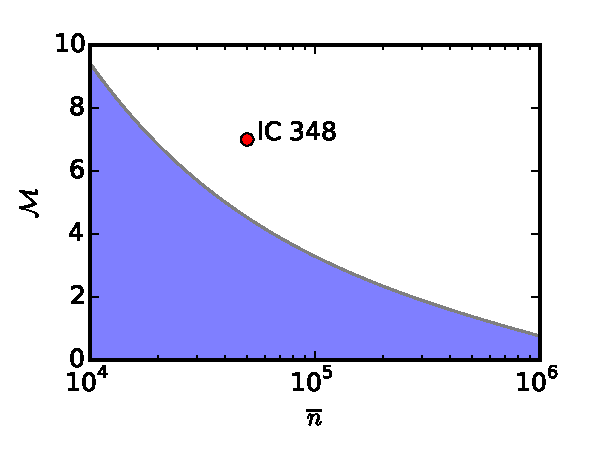
\includegraphics[width=\linewidth]{hw3sol1}
\caption[Solution to problem set~\thesolutionset, problem~\theenumi\theenumii]{
\label{fig:hw3sol1}
Mach number $\mathcal{M}$ versus mean density $\overline{n}$, separating the region where $f(>x_0) < f_{\mathrm{BD}}$ (shaded) from the region where $f(>x_0) > f_{\mathrm{BD}}$. The red point shows the properties of IC 348.
}
\end{marginfigure}
The result is shown as Figure \ref{fig:hw3sol1}. The shaded region is the region where $f(>x_0)<f_{\rm BD}$. Clearly IC 348 (shown as the red dot in the figure) falls into the region where the mass fraction large enough to create brown dwarfs is larger than the brown dwarf mass fraction.

\end{enumerate}

\end{enumerate}